\documentclass[11pt]{article}
\usepackage[margin=1in]{geometry}
\usepackage{amsmath,amssymb}
\usepackage{graphicx}
\usepackage{booktabs}
\usepackage{xcolor}
\usepackage{listings}
\usepackage[colorlinks=true,linkcolor=blue,urlcolor=blue]{hyperref}

\lstset{
  basicstyle=\ttfamily\small,
  keywordstyle=\color{blue!70!black},
  commentstyle=\color{green!40!black},
  stringstyle=\color{red!60!black},
  showstringspaces=false,
  breaklines=true,
  frame=single,
}

\title{A Selectable Precision Backend for \texttt{Teukolsky.jl}:\\
Float64, BigFloat, and MultiFloat}
\author{Teukolsky MST module}
\date{\today}

\newcommand{\Binc}{B^{\mathrm{inc}}}
\newcommand{\bigO}{\mathcal{O}}

\begin{document}
\maketitle

\begin{abstract}
The Mano--Suzuki--Takasugi (MST) solver in \texttt{Teukolsky.jl} computes
homogeneous solutions of the radial Teukolsky equation. Several downstream
quantities---the branch-cut integral of the Green's function and high-multipole
energy fluxes in particular---require many more correct digits than IEEE
double precision provides, while the bulk of the run time is exploratory and
double precision is more than enough. We add a single, uniform \emph{precision
backend} switch that lets the user select \texttt{Float64}, \texttt{BigFloat},
or \texttt{MultiFloat} (the error-free-transform extended precision of
\href{https://github.com/dzhang314/MultiFloats.jl}{\texttt{MultiFloats.jl}}).
Because the MST code is already generic over \texttt{R<:AbstractFloat}, the
integration is additive: a compatibility shim supplies the handful of
transcendental and special functions \texttt{MultiFloats.jl} does not provide,
and a dispatch helper converts inputs to the requested working type. Across a
grid of $\sim 200$ Kerr/Schwarzschild modes the MultiFloat results reproduce a
$512$-bit \texttt{BigFloat} reference to the precision dictated by their limb
count ($\approx 16$ correct decimal digits per \texttt{Float64} limb).
\end{abstract}

\section{Background: where precision matters in MST}

The MST method writes the ``in'' and ``up'' radial Teukolsky solutions as series
of hypergeometric functions indexed by the \emph{renormalized angular momentum}
$\nu$, with expansion coefficients $f^\nu_n$ obeying a three-term recurrence
\cite{ST2003}. Our solver obtains $\nu$ from the monodromy of the confluent Heun
equation: it evaluates $\cos(2\pi\nu)$ as a truncated double series and inverts
the appropriate branch,
\begin{equation}
\cos(2\pi\nu) \;=\; \cos\!\big(\pi(\mu_1-\mu_2)\big)
  \;+\; \frac{2\pi^2}{a_{1,\Sigma}\,a_{2,\Sigma}}\,(-1)^{n-1}\,a_1^{(n+1)}a_2^{(n+1)},
\label{eq:mono}
\end{equation}
where the $a_i^{(k)}$ and the closing sums $a_{i,\Sigma}$ are built from a
truncation-independent recurrence of length $n$. The asymptotic amplitudes then
follow from sums such as
\begin{equation}
A^\nu_+ \;\propto\; \frac{\Gamma(\nu+1-s+i\epsilon)}{\Gamma(\nu+1+s-i\epsilon)}
  \sum_{n} f^\nu_n,
\qquad
\Binc \;=\; \omega^{-1}\big(K_\nu - i\,e^{-i\pi\nu}\,\sigma\,K_{-\nu-1}\big)A^\nu_+\,e^{i\Theta},
\label{eq:amp}
\end{equation}
with the matching coefficients $K_\nu$ involving ratios of $\Gamma$ functions.
The incidence amplitude $\Binc$ controls the Green's function
$G = R_{\mathrm{in}}/(2i\omega\,\Binc)$; cancellations in the branch-cut
contribution and in subdominant flux multipoles can lose $20$--$60$ digits, so a
working precision well beyond $53$ bits is essential there.

\section{Three backends, one switch}

The numerical core (Eqs.~\eqref{eq:mono}--\eqref{eq:amp}) is written generically
in a real type \texttt{R<:AbstractFloat} and its complexification
\texttt{Complex\{R\}}; the precision is therefore fixed entirely by the type of
the inputs $(a,\omega)$. We expose this through a \texttt{backend} keyword on the
public entry points \texttt{compute\_nu} and \texttt{compute\_amplitudes} (and
its \texttt{nufixed}/\texttt{mero} variants):

\begin{center}
\begin{tabular}{@{}lll@{}}
\toprule
\texttt{backend} & working type & precision control \\
\midrule
\texttt{:float64}    & \texttt{Float64}             & fixed, $53$ bits \\
\texttt{:bigfloat}   & \texttt{BigFloat}            & \texttt{precision} bits (arbitrary) \\
\texttt{:multifloat} & \texttt{Float64xN}, $N\le 4$ & \texttt{precision} bits $\to N=\lceil \text{prec}/53\rceil$ limbs \\
\bottomrule
\end{tabular}
\end{center}

A single dispatch helper converts the inputs and runs the otherwise-unchanged
generic path:

\begin{lstlisting}
nu, p  = compute_nu(s, l, m, a, omega; backend=:multifloat, precision=212)
amps   = compute_amplitudes(s, l, m, a, omega; backend=:multifloat, precision=212)
\end{lstlisting}

The default (\texttt{:auto} on the amplitude routines, \texttt{:bigfloat} on
\texttt{compute\_nu}) reproduces the previous behaviour byte-for-byte, so the
change is fully backward compatible.

\section{What MultiFloat is, and the two caveats it forces}

A \texttt{MultiFloat\{Float64,N\}} (alias \texttt{Float64xN}) represents a number
as an unevaluated sum of $N$ nonoverlapping \texttt{Float64} values and
implements $+,-,\times,\div,\sqrt{\,}$ with error-free transforms, delivering
$\approx 53N$ bits of \emph{mantissa} at a few times the cost of hardware
double precision---typically far faster than \texttt{BigFloat} for
arithmetic-dominated kernels \cite{MultiFloats}. Two properties of this design
shape the integration:

\paragraph{(C1) Mantissa, not exponent.} A \texttt{MultiFloat} extends the
significand but keeps \texttt{Float64}'s exponent range
($\sim 10^{\pm 308}$). The monodromy series \eqref{eq:mono} accumulates
factorial/Pochhammer products whose magnitude overflows to \texttt{Inf}/\texttt{NaN}
at series length $n\gtrsim 170$---exactly the reason the \texttt{Float64} path is
capped at $n=60$. At extended precision the required length grows as
$n\approx 4.7\times(\text{bits})$, far past the overflow point. We therefore
evaluate the \emph{scalar} $\cos(2\pi\nu)$ of \eqref{eq:mono} in \texttt{BigFloat}
at the MultiFloat working precision and convert the single result back; the
arithmetic-heavy remainder (the $f^\nu_n$ recurrence and the amplitude/$K_\nu$
sums, whose terms stay within the exponent range) runs natively in MultiFloat.

\paragraph{(C2) Missing transcendentals / $\Gamma$.}
\texttt{MultiFloats.jl} does not implement the elementary transcendentals or the
$\Gamma$ function. A compatibility shim (\texttt{src/multifloat\_compat.jl},
mirroring the existing \texttt{arb\_compat.jl}) closes the gaps used by MST:
\begin{itemize}
  \item it enables MultiFloats' sanctioned \texttt{BigFloat} fallback for the
        one-argument transcendentals ($\sin,\cos,\exp,\log,\dots$);
  \item it adds the \emph{two}-argument $\operatorname{atan}(y,x)$ that the
        fallback omits but on which \texttt{Complex} $\log/\arccos/\operatorname{arccosh}$
        depend;
  \item it adds $\Gamma$ on \texttt{Complex\{MultiFloat\}} (routed through
        \texttt{BigFloat} at the working precision), as in
        Eq.~\eqref{eq:amp}.
\end{itemize}
These functions appear only $\bigO(1)$ times per call (prefactors and branch
selection), so the \texttt{BigFloat} detour is negligible while the dominant
arithmetic stays native.

\paragraph{Width limit.} The shipped \texttt{MultiFloats.jl} provides
multiplication/division/square-root kernels only for $N\le 4$
(\texttt{Float64x1}\,$\ldots$\,\texttt{Float64x4}), so the MultiFloat backend tops
out at $\approx 212$ bits ($\approx 63$ decimal digits); request more digits via
the \texttt{:bigfloat} backend. The precision$\to$width map clamps accordingly.

\section{Validation}

Figure~\ref{fig:acc} shows the relative error of $\nu$ and $\Binc$ for a
representative Kerr mode against a $1024$-bit \texttt{BigFloat} reference, as a
function of working precision. The MultiFloat points (blue) lie on top of the
\texttt{BigFloat} curve (gray) at every matching bit count, each additional limb
buying $\approx 16$ decimal digits, until the $N=4$ ceiling. \texttt{Float64}
(red) sits at the $\sim 10^{-11}$ level set by the conditioning of this mode.

\begin{figure}[h]
\centering
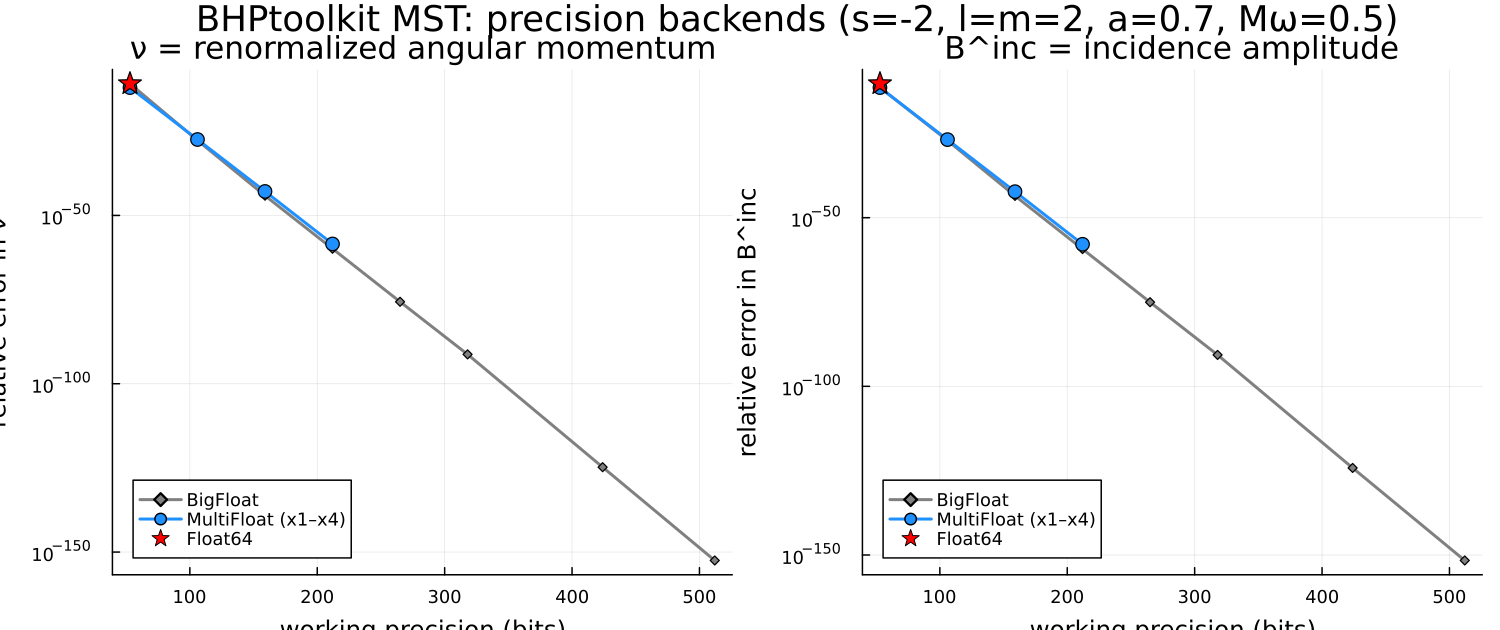
\includegraphics[width=\textwidth]{multifloat_accuracy.png}
\caption{Relative error of the renormalized angular momentum $\nu$ (left) and the
incidence amplitude $\Binc$ (right) versus working precision, for
$s=-2,\ \ell=m=2,\ a=0.7,\ M\omega=0.5$, against a $1024$-bit \texttt{BigFloat}
reference. MultiFloat (blue, $N=1\ldots4$) matches \texttt{BigFloat} (gray) at
equal bit width; \texttt{Float64} (red) is shown for scale.}
\label{fig:acc}
\end{figure}

\begin{table}[h]
\centering
\begin{tabular}{@{}lrr@{}}
\toprule
backend / width & bits & rel.\ error in $\nu$ \\
\midrule
\texttt{Float64}          & 53  & $1.3\times10^{-11}$ \\
\texttt{Float64x2}        & 106 & $3.6\times10^{-28}$ \\
\texttt{Float64x3}        & 159 & $1.3\times10^{-43}$ \\
\texttt{Float64x4}        & 212 & $3.4\times10^{-59}$ \\
\texttt{BigFloat} (212)   & 212 & $1.3\times10^{-60}$ \\
\bottomrule
\end{tabular}
\caption{Accuracy scaling for the mode of Fig.~\ref{fig:acc}: each MultiFloat
limb adds $\approx 16$ correct decimal digits, matching \texttt{BigFloat} at the
same bit width.}
\label{tab:scaling}
\end{table}

A broader sweep of $\sim 200$ modes (spins $a\in\{0,0.5,0.9,0.99\}$, several
$(\ell,m)$, and real and complex $\omega$) confirms: every MultiFloat result is
finite, beats \texttt{Float64}, and reproduces the \texttt{BigFloat} reference to
the expected precision. The dedicated test set lives in
\texttt{test/test\_multifloat\_backend.jl}.

\section{Summary}

The MST solver now offers a uniform three-way precision option. \texttt{Float64}
is the fast default; \texttt{BigFloat} provides unbounded precision for the most
demanding branch-cut/flux computations; and \texttt{MultiFloat} occupies the
useful middle ground of $30$--$60$ extra-precise digits with native,
non-allocating arithmetic, while delegating only its missing transcendentals and
the overflow-prone monodromy scalar to \texttt{BigFloat}.

\begin{thebibliography}{9}
\bibitem{ST2003} M.~Sasaki and H.~Tagoshi,
  \emph{Analytic Black Hole Perturbation Approach to Gravitational Radiation},
  Living Rev.\ Rel.\ \textbf{6} (2003) 6.
\bibitem{MultiFloats} D.~K.~Zhang, \texttt{MultiFloats.jl},
  \url{https://github.com/dzhang314/MultiFloats.jl}.
\end{thebibliography}

\end{document}
